\newpage
\section{Aufbau und Durchführung}
\subsection{Aufbau}
\label{sec:Aufbau}
    \begin{figure}[ht]
        \centering\captionsetup{format=plain}
        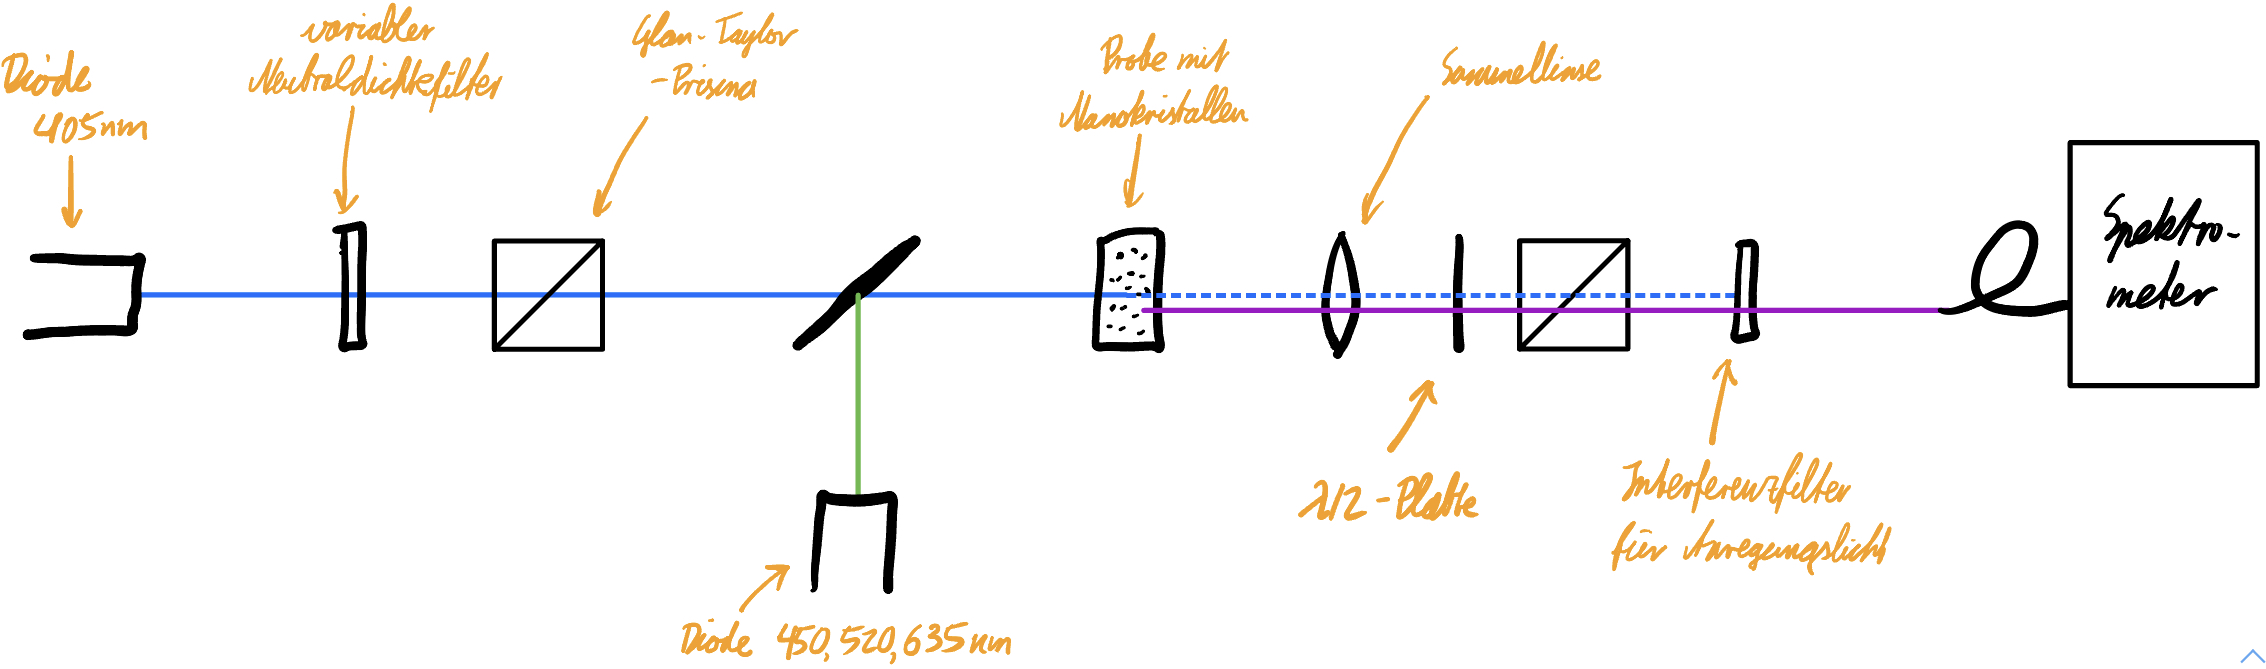
\includegraphics[width=0.9\textwidth]{bilder/Aufbau.jpeg}
        \caption{Hier ist der schematische Aufbau des Photolumineszenzversuches dargestellt. \cite{anleitung}}
        \label{fig:Aufbau}
    \end{figure}
    \FloatBarrier
    Als Anregungslaser werden Diodenlaser benutzt.
    Dazu sind zwei Strahlarme aufgebaut.
    Der Erste besteht aus einer \qty{405}{nm}-Laserdiode deren Leistung verstellt werden kann, einem variierbaren Neutraldichtefilter (ND-Filter), der eine einfachere Veränderung der Laserleistung ermöglicht und einem Glan-Taylor-Prisma zur Polarisierung des Lichtstrahls.
    Beim Anderen werden Diodenlaser der Wellenlängen 450, 520 und \qty{635}{nm} eingesetzt und auf einen dichroitischen Spiegel eingestellt, der Licht unterhalb \qty{425}{nm} transmitiert und Licht oberhalb reflektiert.
    Dieser Aufbau ermöglicht ein schnelles Wechseln des für die Messung benutzten Anregungslasers, durch einfaches An- und Ausschalten.

    Es werden drei Proben von in Toluol gelösten verschieden großen kolloidalen Nanokristallen aus CdSe in den Strahlengang gestellt, sodass Photolumineszenz entsteht.
    Eine vierte Probe enthält Kohlenstoff-Quantenpunkte.
    Im Anschluss wird das Photolumineszenzlicht durch eine Sammellinse kollimiert und durch eine $\lambda/2$-Platte, als auch ein Glan-Taylor-Prisma und einen Interferenzfilter zum herausfiltern des Anregungslichtes geschickt.
    Das resultierende Licht wird über eine Glasfaser in ein Spektrometer eingekoppelt, welches mit einem Computer verbunden ist und das Frequenzspektrum des Lichtes in Echtzeit darstellt.
    Um das Rauschen zu verringern kann die Integrationszeit hochgestellt werden.
    In der \autoref{fig:Aufbau} ist dies nicht dargestellt worden, jedoch wird der Aufbau nach der Probe unter einem Winkel aufgestellt, sodass Reflektionen des Anregungslichtes noch weiter minimiert werden.
    
    
\subsection{Durchführung}
\label{sec:Durchfuehrung}
    Zuerst wurde der Strahlengang wie in \autoref{sec:Aufbau} dargelegt aufgebaut.
    Danach wurde der \qty{405}{nm}-Laser bei einer Leistung von \qty{1}{mW} verwendet, um die Spektren aller vier Proben aufzunehmen.
    Als Nächstes wurde die Kombination der $\lambda/2$-Platte und des Glan-Taylor-Prismas zur Untersuchung der linearen Polarisation der Photolumineszenzsstrahlung genutzt.
    Dabei wurde ein Spektrum für einen Winkel von 0° zwischen den optischen Achsen der Verzörgerungsplatte und des Prismas und ein Spektrum für einen Winkel von 90°.
    Um die Abhängigkeit der Photolumineszenz-Signale von der Laserleistung zu betrachten wurde die Intensität des Lasers mit dem ND-Filter variiert und dabei PL-Spektren aufgenommen.
    Zur Einstellung der benutzten Laserleistung wurde ein Detektor zwischen den dichroitischen Spiegel und die Probe gestellt.
    Zum Schluss wurden die PL-Spektren wie bei der ersten Messung mit den anderen drei Lasern aufgenommen.

    Aufgrund der nicht-rotationssymmetrischen Grundfläche der Quarzfläschchen wurden diese bei jeder Messung so gedreht, dass das Photolumineszenzignal so groß wie möglich und das zu den Reflektionen des Lasers gehörende Signal so klein wie möglich sei.
